\chapter{Experimentos Computacionais}
Para a realização do experimentos computacionais foi necessário, primeiramente, obter os dados para teste e organizá-los para posteriormente submeter ao modelo para geração dos hiperplanos classificadores  e aos testes de classificação. Todos os experimento foram feitos utilizando um notebook com processador Intel Core i3, 2.27 GHz, 3 GB de RAM, sistema operacional Ubuntu 12.04, NetBeans IDE 7.1.2 e o software CPLEX da IBM.

Todo o processo, desde a organização dos dados até a etapa de classificação, foi implementado utilizando a linguagem de programação Java. A implementação foi feita em módulos, organizados da seguinte forma: Módulo organizador de dados, Módulo de geração de classificadores, Módulo de classificação, Módulo validador. No módulo organizador de dados os conjutnos de dados são organizados em subgrupos, cada subgrupo contendo vetores de todos os padrões, essa organização é importante para a etapa de validação do método. No Módulo de geração de classificadores está implementado o modelo de programação linear e são gerados os hiperplanos separadores. Os Módulos de classificação e validador são utlizados na etapa de teste, o primeiro realiza a classificação de de um vetor em um dos padrões separados pelo hiperplano e o segundo realiza a validação do método de reconhecimento de padrões utlizando o método cross validation.

Na figura \ref{img:diagrama_modulos} estão representadas as principais etapas realizadas durante os experimentos computacionais.

\begin{center}
	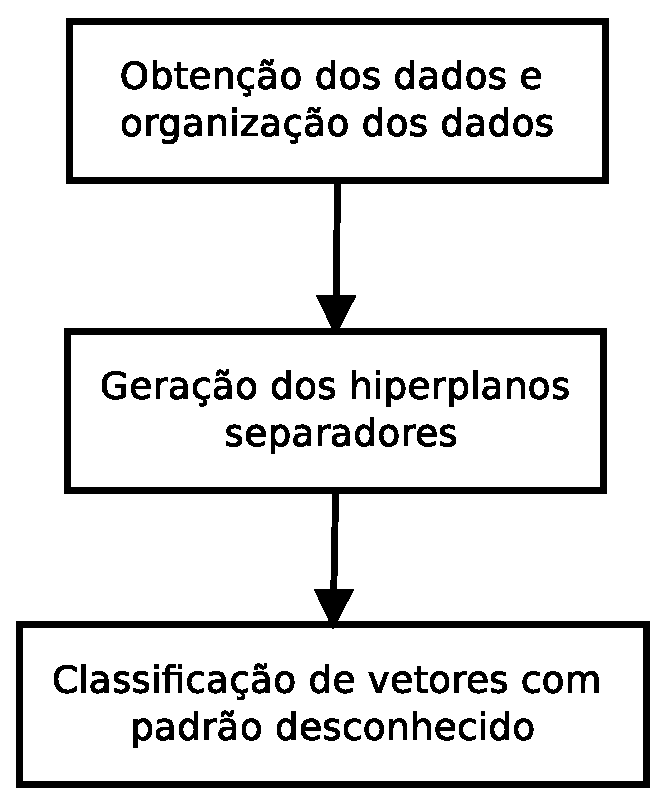
\includegraphics[scale=0.5]{graficos/diagrama_modulos}
	\captionof{figure}{Diagrama simples das etapas realizadas nos experimentos}
	\label{img:diagrama_modulos}
\end{center}

Primeiramente os dados foram obtidos já no formato de vetores de caracteríticas ou extraídos de imagens, e depois foram divididos em subgrupos. Em seguida foram submetidos ao modelo de Programação Linear, reponsável por gerar os classificadores e por último vetores com padrão desconhecido foram classificados. As duas últimas etapas são repetidas a cada ciclo de teste, essas repetições são controladas pelo Módulo validador. Nas seções seguintes essas etapas serão apresentadas de forma mais detalhada.

\section{Conjuntos de Dados}
Foram relaizados testes com quatro conjuntos de dados: dígitos de 0 a 9 escritos manualmente, gestos da Língua Brasileira de Sinais, espécies da planta Iris e expressões facias . Desses conjuntos, os três primeiros foram obtidos do repositório de dados \citeonline{Repositorio2013} e já estavam representados na forma de vetores de características. O último conjunto foi gerado a partir do conjunto de imagens JAFFE \cite{Jaffe}. A seguir são apresentadas as caraterísticas de cada um dos quatro conjuntos de dados:

\begin{itemize}
\item \textbf{Dígitos de 0 a 9 escritos manualmente \cite{Digitos}}
Na formação desse conjunto de dados 250 digítos entre 0 e 9 foram escritos de forma aleatória por 44 pessoas, totalizando 11000 dígitos, porém estão disponíveis 10992 dígitos. Durante a coleta dos dados foram recolhidas, em intervalos fixos de 100 milisegundos, as coordenadas e a pressão da caneta sobre a superfície enquanto o dígito era escrito. No conjunto de dados utilizada foram considerados apenas os valores das coordenadas. Os dados foram reorganizados utilizando interpolação linear, foram utilizados 8 pontos, e obtidos vetores com 16 características.
Cada vetor é composto por 16 atributos que variam entre 0 e 100 e mais um valor variando entre 0 e 9 que representa o classe a qual o vetor pertence.
Os dados estão distribuídos como na tabela a seguir:
\begin{center}
	\begin{tabular}{cc}
        \hline
        Classe & Quantidade de instâncias \\
        \hline
		0 & 1143 \\
		1 & 1143 \\
		2 & 1144 \\
		3 & 1055 \\
		4 & 1144 \\
		5 & 1055 \\
		6 & 1056 \\
		7 & 1142 \\
		8 & 1055 \\
		9 & 1055 \\
        \hline
	\end{tabular}
	\label{tab:tabela_digitos}
        \captionof{table}{Quantidade de instâncias de cada dígito}
\end{center}

\item\textbf{Gestos da Língua Brasileira de Sinais (LIBRAS) \cite{Libras}}
Esse conjunto de dados é composta por 15 classes, ou seja, nela estão presentes 15 sinais da LIBRAS, sendo 24 instâncias de cada classe, totalizando 360 vetores de características. Os dados foram extraídos de vídeos com tempo médio de 7 segundos, em cada vídeo um movimento é executado e depois é representado como uma curva bidimensional. No pre processamento foram selecionados 45 frames de cada vídeo, em cada frame a coordenada do ponto central da mão é encontrado, compondo uma curva com 45 pontos. As coordenadas dos 45 pontos formam o vetor de características com 90 valores, os 45 primeiros valores representam o valor de x e o restante o valor de y.
O vetor de características tem no total 91 valores, sendo que 90 deles caracterizam o movimento e o último valor representa o padrão ao qual o vetor pertence.

\item \textbf{Espécies da planta Iris \cite{Iris}}
Nesse conjunto de dados são representados três tipos da planta Iris, é composta por 50 instâncias de cada tipo, totalizando 150 vetores. Cada vetor é composto por 4 características: comprimento da sépala, largura da sépala, comprimento da pétala, largura da pétala; e mais o nome da classe que o vetor representa.

\item \textbf{Expressões facias}
No caso das expressões faciais, as imagens foram obtidas do conjunto de dados JAFFE \cite{Jaffe} e o pre processamento e a extração e caracteríticas foram implementaos na linguagem de programação Python.
Inicialmente a proposta do presente trabalho era focar apenas na classificação de expressões faciais utilizando a programação linear. Durante a pesquisa não foi encontrada nenhum conjunto de dados que disponibilizasse os vetores de características da imagens, portanto foi necessária a implementação para a obtenção dos dados. Posteriormente foi verificado que seria necessário um aprofundamento do estudo na área da visão computacional, para que os vetores de caracteríticas não comprometessem o método classificador. Portanto esses dados foram obtidos através de uma implementação superficial de extração de caracteríticas.
Após a obtenção do banco de imagens JAFFE. As imagens foram recortadas a fim de isolar a região da face, utilizando linguagem de programação python, como mostrado na figura

\begin{center}
	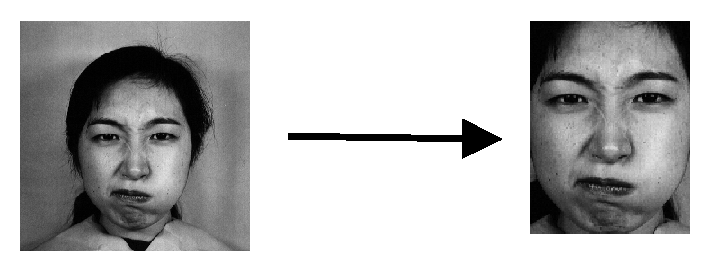
\includegraphics[scale=0.5]{graficos/jaffe}
	\captionof{figure}{Pre processamento das imagens do banco JAFFE}
	\label{img:jaffe}
\end{center}

O banco de imagens JAFFE é composto por 213 imagens, sendo divididas em 7 expressões: tristeza, alegria, desgosto, surpresa, raiva, medo e neutro. Na tebela \ref{tab:tabela_expressoes} é apresentada a quantidade de imagens para cada expressão.

\begin{center}
	\begin{tabular}{cc}
        \hline
        Classe & Quantidade de imagens \\
        \hline
		Tristeza & 31 \\
		Alegria & 31 \\
		Desgosto & 29 \\
		Surpresa & 30 \\
		Raiva & 30 \\
		Medo & 32 \\
		Neutro & 30 \\
        \hline
	\end{tabular}
	\captionof{table}{Quantidade de imagens para cada expressão}
        \label{tab:tabela_expressoes}
\end{center}

Na extração dos vetores de características foi utilizado o método Local Binary Patterns (LBP) que é um classificador de texturas. A cada pixel da imagem é atribuído um código, que é gerado a partir dos pixels ao redor. Tomando como referência o pixel central, a cada pixel vizinho é atribuído o valor 0 ou 1: se o valor do pixel vizinho for menor que o valor do pixel central, o valor 0 é atribuído, se for menor, o valor atribuído é 1. A partir daí, é gerado um código binário que é transformado em um valor decimal, esse valor decimal é o código LBP do pixel central \cite{LBPShan2009}. A figura abaixo demonstra como é calculado o código LBP.

\begin{center}
	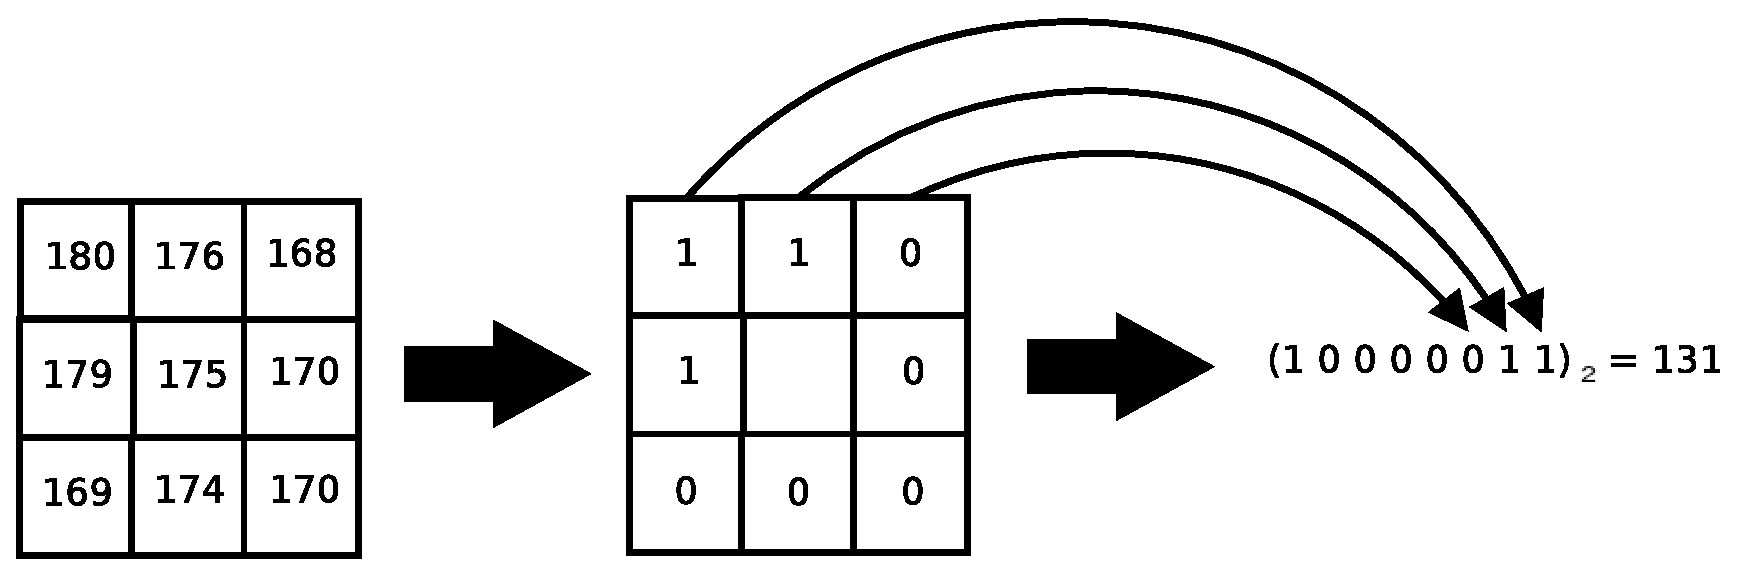
\includegraphics[scale=0.5]{graficos/LBP}
	\captionof{figure}{Cálculo do código LBP}
	\label{img:LBP}
\end{center}

Na implementação, primeiramente, a imagem é dividida em blocos, é gerado o histograma dos códigos LBP de cada bloco, por fim, os histogramas são concatenados. Esse resultado final é o descritor de texturas da imagem. A figura \ref{img:LBPHistograma} representa esse processo.

\begin{center}
	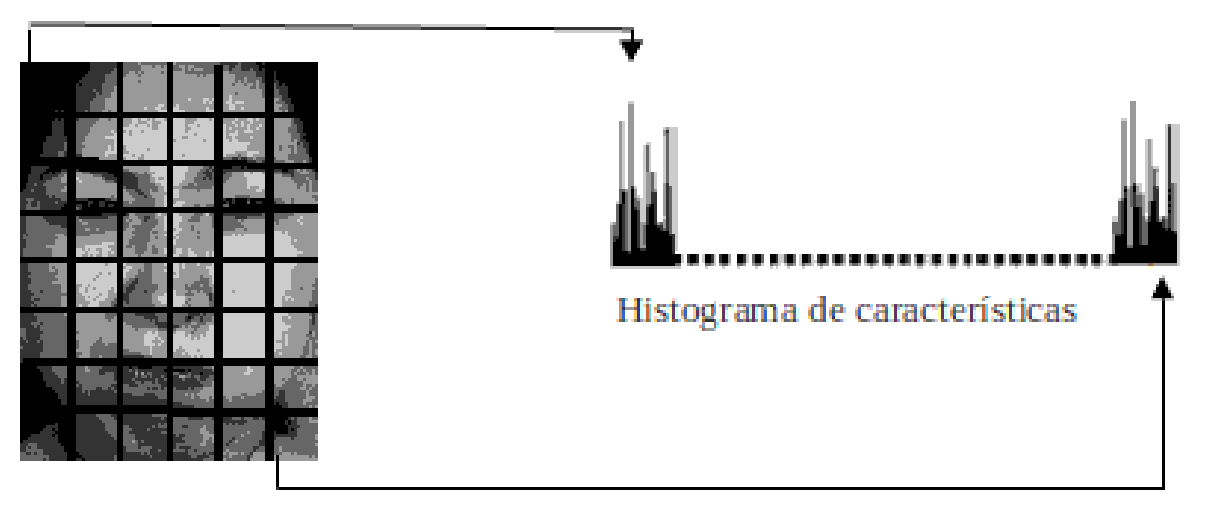
\includegraphics[scale=0.5]{graficos/histograma}
	\captionof{figure}{Representação da imagem dividida em blocos e da concatenação dos histogramas de cada bloco.}
	\label{img:LBPHistograma}
\end{center}

Para reduzir o tamanho do vetor de caracteríticas os códigos LBP de cada pixel são somados e divididos pelo número de imagens, qundo o resultado é menor do que um valor limiar os códigos desse pixel é excluído em todos os vetores \cite{Feng}. O limiar adotado nese caso foi 5 \cite{LBPShan2009}. Resultando em vetores de tamanho 843, sendo composto por 842 caracteríticas mais um dígito identificador do padrão. 
\end{itemize}

Nos vetores de características de todos os conjuntos de dados utlizados, é acrescido um valor informando a classe representada pelo vetor, para as etapas de treinamento e teste esse valor é omitido, ele só é utlizado na etapa de validação para verificar se o vetor foi corretamente classificado.

\section{Organização dos dados}
Em todos os testes foi o utilizado o método k -fold cross validation com k = 10, em seus trabalhos \citeonline{Baldisserotto05Validacao}, \citeonline{Kohavi95Cross}, \citeonline{Guo} utlizaram esse mesmo parâmetro. Os dados foram dividos em 10 subgrupos com mesmo tamanho \cite{Guo} e com a mesma quantidade de vetores para cada classe, por isso não foram em utlizados todos os dados de todos os conjuntos de dados.

\begin{center}
	\begin{tabular}{|p{2cm}|p{3cm}|p{2cm}|p{2cm}|}
        \hline
        \multicolumn{4}{|c|}{Conjuntos de dados} \\ \hline
        Nome & Total de vetores & Vetores utilizados & Quantidade de padrões\\ \hline
		Dígitos    &10992  & 10500 & 10\\ \hline
		LIBRAS     & 360   & 300   & 15\\ \hline
		Íris       & 150   & 150   & 3\\ \hline
		Expressões & 213   & 210   & 7\\ \hline
	\end{tabular}
        \captionof{table}{Organização dos dados}
	\label{table:org_dados}
\end{center}

Na tabela \ref{table:org_dados} constam informações dos quatro conjuntos de dados utlizadas como teste nomeadas da seguinte forma: Dígitos, LIBRAS, Íris, Expressões. Na segunda coluna são apresentados quantos vetores compõem o conjunto de dados no total sem distinguir o número de vetores por classe. E na última coluna são apresentados o número de vetores utlizados nos testes, em todos os casos o núemro de vetores utlizados é divisível por 10 por ser utlizado o parâmetro k = 10.

No conjunto de dados Dígitos, as classes que possuiam menos vetores eram as dos dígitos 3, 5, 8 e 9 com 1055 vetores, e as que possuiam mais vetores eram as dos dígitos 2 e 4 com 1144 vetores como mostrado na tabela \ref{tab:tabela_digitos}. Nessa caso, foram utilizados 1050 vetores de cada classe, totalizando 10500 vetores.

No conjunto de dados LIBRAS, cada classe possui 24 vetores, para a distribuição dos vetores entre os 10 subgrupos foram utlizados 20 vetores de cada classe, totalizando 300 vetores.

O conjunto de dados Íris possui 50 vetores para cada classe, possibilitando a utlização dos 150 vetores na distribuição entre os 10 subgrupos.

No quarto conjunto de dados, Expressões, a classe desgosto possui 29 vetores enquanto as classe restantes possuem 30 ou mais, como mostrado na tebela \ref{tab:tabela_expressoes}. Nesse caso, uma imagem da classe desgosoto foi repetida e utilizou-se 30 vetores para cada classe. 

Para esse conjunto de dados Expressões, se vetores fossem excluídos em todas as classes, o número de vetores divisível por 10, que é a quantidade de subgrupos, mais próximo é 20, o que acarretaria a exclusão de 9 ou mais imagens por classe, em contrapartida, na solução utlizada apenas 1 ou 2 imagens foram excluídas de cada classe, com exceção da classe desgosto que teve apenas uma imagem repetida. Já no conjunto de dados Dígitos optou-se pela exclusão, pois seria necessário repetir muitos vetores nas classes com o número mais baixo de vetores, o que poderia comprometer o resultado, o mesmo ocorre com o conjunto de dados LIBRAS.

\section{Resultados}
Nesta seção são apresentados os resultados encontrados nos testes realizados com os quatro conjuntos de dados anteriormento descritos. 

Na tabela a seguir são apresentados os resultados dos quatro conjuntos de dados após a validação 10-fold cross validation, a taxa de acerto é uma média das taxas obtidas em cada um dos 10 ciclos de teste. 

\begin{center}
	\begin{tabular}{|c|c|c|c|c|c|c|c|}
        \cline{1-7}
        \multicolumn{4}{ |c| }{Conjunto de dados} & \multicolumn{3}{ c| }{Vetores por padrão} \\
        \hline 
	Nome & Quantidade de   & Total de & Total & No          & Na & Taxa de\\ 
         ~   & características & vetores  &  ~    & treinamento & classificação & acerto (\%)
        \\  \hline
    	Dígitos    &        16     & 10500  & 1050 & 945   & 105 & 98\\ \hline
   	LIBRAS     &        90     &   300  &   20 &  18   &   2 & 72\\ \hline
    	Íris       &         4     &   150  &   50 &  45   &   5 & 87\\ \hline
    	Expressões &       842     &   210  &   30 &  27   &   3 & 34\\ \hline
	\end{tabular}
        \captionof{table}{Resultados após a validação 10-fold cross validation}
	\label{tab:resultados}
\end{center}

Na tabela \ref{tab:resultados} é aprsentada a quantidade de caracetrísticas presente em cada vetor de cada conjunto da dados, a quantidade de vetores de cada classe utilizados para treinamento e a quantidade de vetores de cada classe utilizados para teste a cada ciclo da validação cruzada. Na última coluna é apresentada a taxa média de classificações corretas ao final da validação.

Nessa tabela é possível observar que as classe com menos caracteríticas obtiveram as maiores taxas de acertos. Comparando os dois conjuntos com maioires taxas, observamos que o conjunto Dígitos com um número de vetores muito superior a do conjunto Íris obteve a maior taxa de acerto. O conjunto de dados Expressões, apesar de possuir uma quantidade de vetores superior a da classe LIBRAS, a quantidade de caracteríticas que é um número muito superior e possui a taxa de acerto mais baixa. 

Na tabela a seguir são apresentadas as taxas de acerto em cada ciclo de teste.

\begin{center}
	\begin{tabular}{|c|c|c|c|c|c|c|c|c|c|c|}
        \hline
        \multicolumn{1}{ |c| }{Conjunto} & \multicolumn{10}{ c| }{Taxas de acertos por ciclo de teste (\%)}
        \\ \cline{2-11}
	de dados  & C 1 & C 2 & C 3 & C 4 & C 5 & C 6 & C 7 & C 8 & C 9 & C 10 \\ \hline
    	Dígitos   & 0,98 & 0,98 & 0,98 & 0,98 & 0,98 & 0,98 & 0,98 & 0,97 & 0,96 & 0,97\\ \hline
   	LIBRAS    & 0,4  & 0,77 & 0,74 & 0,7 & 0,63 & 0,7  & 0,63 & 0,83  & 0,93 & 0,9 \\ \hline
    	Íris      & 0,74 & 0,8  & 0,93 & 0,87 & 0,93 & 0,74 & 0,87 & 0,87 & 0,93 & 0,87\\ \hline
    	Expressões& 0,34 & 0,38 & 0,38 & 0,33 & 0,29 & 0,29 & 0,24 & 0,43 & 0,33 & 0,43\\ \hline
	\end{tabular}
        \captionof{table}{Taxas de acerto em cada ciclo de teste}
	\label{tab:taxas}
\end{center}

Na tabela \ref{tab:taxas} pode ser observado que nos dados Dígitos houve menos variação na taxa. Nos dados Íris houve certa variação entre 74\% e 93\%. Os dados LIBRAS e Expressões, que são os que possuem os maiores vetores apresentaram uma maior varaiação. 

\subsection{Quantidade de vetores X Taxa de acerto}
Os conjuntos de dados são compostos por mais de um vetor de características de cada classe, e a quantidade de vetores pode influênciar na taxa de acertos final. Para fazer essa análise foi utilizado o banco de dados Dígitos por ser, entre os conjuntos utlizados, o que contém o maior número de vetores por classe.

\begin{center}
	 \begin{tabular}{|c|c|c|c|}
    \cline{1-3}
    \multicolumn{3}{|c|}{\textbf{Conjunto de dados Dígitos}}                     \\ \cline{1-3}
    \multicolumn{3}{|c|}{Vetores por padrão}                    \\ \hline
    Total                     & No treinamento & Na classificação & Taxa de \\ ~                         & ~              & ~                & acerto ( \% ) \\ \hline

    	   50   & 	45		   &		5	& 	0.898\\ \hline
   	  100   & 	90		   &	       10	&	0.926\\ \hline
	  200   &      180   		   &	       20	&	0.947\\ \hline
    	  300 	&      270		   &	       30	&	0.964\\ \hline
    	  500 	&      450  		   & 	       50	&	0.968\\ \hline
    	  600 	&      540		   &	       60	&	0.972\\ \hline
    	  900 	&      810		   &	       90	&	0.974\\ \hline
    	 1000 	&      900		   &	      100	&	0.975\\ \hline
    	 1050 	&      945		   &	      105	&	0.975\\ \hline
	\end{tabular}
        \captionof{table}{Quantidade de Vetores X Taxa de acerto}
	\label{tab:vetorxtaxa}
\end{center}

Na primeira coluna da tabela \ref{tab:vetorxtaxa} estão específicadas as quantidades de vetores de cada classe e nas duas colunas seguintes as quantidades de vetores de cada classe utilizados na etapa de treinamento e na etapa de testes respectivamente. Na útlima coluna estão específicadas as taxas de acertos em cada teste. 

É possível observar um aumento na taxa de acertos a medida que a quantidade de vetores cresce. Porém esse aumento não é proporcional ao aumento do núemro de vetores. A variação na taxa de acerto diminui a medida que a quantidade de vetores aumenta, do teste com 50 vetores por calsse para o teste com 100, houve uma variação de 2,8\% na taxa de acerto. Já no testes com 200 e 400 a variação na taxa foi de 2\%. E entre o teste com 600 vetores e o teste com quantidade máximamde vetores que é 1050 é observado uma variação bem pequena de 0,02\% na taxa de acerto.

\subsection{Tempo computacional}
A partir dos testes realizados também foram realizadas análises do ponto de vista computacional.
Os resultados mostrados na tabela a seguir são as médias dos tempos de 5 execuções incluindo a etapa de validação compĺeta, com os dez ciclos .

\begin{center}
\begin{tabular}{|c|c|c|c|c|c|}
\hline
\multicolumn{3}{ |c| }{Conjuntos de dados} & \multicolumn{3}{ c| }{Tempo de execução (em segundos)} \\ \hline
Nome       & Quantidade & Vetores & Gerador de  & Gerador de  & Treinamento  \\ 
  ~        &     de     &    por  & hiperplanos & hiperplanos &     e        \\
  ~        &  padrões   &  padrão & por ciclo   & total       & Classificação \\   \hline
Dígitos    &     10     &  1050   &   2,18      &   21,88     &    30,53 \\ \hline
Libras     &     15     &    20   &   0,65      &    6,47     &     7,87 \\ \hline
Iris       &      3     &    50   &   0,04      &    0,41     &     0,65 \\ \hline
Expressões &      7     &    30   &   0,78      &    7,82     &     8,93 \\ \hline


\end{tabular}
        \captionof{table}{Tempos computacionais}
	\label{tab:tempocomp}
\end{center}

Na terceira linha da tabela \ref{tab:tempocomp} estão os tempos de execução apenas do módulo de geração de classificadores, que é o módulo onde o modelo de programação linear é resolvido. É possível constatar um tempo computacional para a geração dos classificadores corresponde a mais de 50\% do tempo computacional total. A quantidade de classificadores gerados deve ser considerada. Na quinta coluna é apresentado o tempo médio para geração dos classificadores a cada ciclo de teste e na segunda linha da tabela são apresentadas as quantidades de classificadores gerados nesse tempo, para três conjuntos de dados esse tempo foi inferior a 1 segundo.

Na última linha da tebla \ref{tab:tempocomp} são apresentados os tempos totais de execução de cada experimento. Pode-se constatar que esse tempo é proporcional ao tamanho dos vetores do conjunto de dados e a quantidade de classes. O conjunto de dados Íris obteve um tempo computacional menor que 1 segundo sendo um conjunto de dados com 3 classe e 50 vetores para cada classe. Enquanto o conjunto de dados Dígitos obteve o maior tempo computacional apesar de possuir vetores com 16 caracteríticas é o conjunto de dados com maior número de vetores por classe. 

Comparando os tempos computacionais dos conjuntos Dígitos e Expressões é possível verificar que a quantidade de vetores por classe teve maior influência no tempo de execução, já que a diferença dos tempos de execução das duas classes é bastante alto, proporcional a diferença entre as quantidades de vetores por classe. 

A mesma observação pode ser feita comparando os tempos dos conjuntos LIBRAS e Expressões, ainda que o número de classe do conjunto LIBRAS seja mais que o dobro do número de classes do conjunto Expressões, cada vetor do conjunto Expressões possui muitas características a mais que os vetores do conjunto LIBRAS e o tempo computacional do conjunto Expressões foi superior ao tempo do conjunto LIBRAS.

\section{Análise dos Resultados}

Juntamente com o conjunto de dados Dígitos \cite{Digitos}, estão disponíveis resultados de testes utilizando como metódo de classificação K nearest neighbor, a métrica utlizada para medir as distâncias entro os K vizinhos mais próximos foi a distância Euclidiana. O autor testou variando o parâmetro K de 1 à 11 com a taxa de acerto variando entre 97,34\% e 97,80\%. Em relação ao experimentos realizados neste trabalho é possível verificar que utilizando o método proposto foram obtidas taxas de acertos próximas as encontradas em \citeonline{Digitos}.

Em seu trabalho \citeonline{Swan2012Iris} abordou a classificação de padrões utlizando Redes Neurais e o conjunto de dados Íris. O autor dividiu 75 vetores para treinamento e 75 para teste. Foram realizados 3 testes, variando um parâmetro na configuração da rede neural. As taxas de acertos obtidas variaram entre 83,33\% e 96,66\%. No experimento utilizando o modelo de programação linear a media de acertos obtida foi de 87\%, um taxa que supera a obtida utilizando redes neurais, dependeno da configuração.

Em \citeonline{Feng} foi utilizado o conjunto de dados JAFFE \cite{Jaffe}. O modelo de programação linear proposto em \citeonline{Bennett92robustlinear} é utlizado para gerar os classificadores e na classificação de imagens com expressão desconhecida foi utilizada uma árvore de torneio, assim como nos experimentos deste trabalho. A taxa de acerto foi de 93.8\%.

No trabalho de \citeonline{Guo} também foi utilizado o banco JAFFE \cite{Jaffe}. Foram feitas comparações entre aluns métodos de classificação, entre eles: Bayes com taxa de acertos 71,0\%, Support Vector Machine linear e não linear, com taxa de acertos 92,4\% e 91,9\%, respectivamente e uma variação do modelo de programação linear utilizado neste trabalho, com taxa 91,0\%. Em todos os casos foram utilizados mecanismos para seleção das características que seriam utlizadas
 
Tanto no trabalho de \citeonline{Feng} quanto no trabalho de \citeonline{Guo} foram obtidas taxas consideravelmente mais altas do que a obtida nos experimentos (34,0\%). Essa diferença pode ser atribuída pela falta de pre processamento das imagens, como já comentado anteriormente.
